\documentclass[oneside,final,14pt]{extreport}
\usepackage[utf8]{inputenc}
\usepackage[russianb]{babel}
\usepackage{vmargin}
\setpapersize{A4}
\setmarginsrb{2cm}{2cm}{3cm}{1.5cm}{0pt}{0mm}{0pt}{14mm}
\usepackage{indentfirst}
\usepackage{amsmath}
\usepackage{graphicx}
\usepackage{verbatim}
\usepackage{hyperref}
\usepackage{listings}
\newcommand{\tocsecindent}{\hspace{7mm}}

\lstset{
   breaklines=true,
   basicstyle=\ttfamily}
\sloppy
\begin{document}
\begin{titlepage}
\newpage
\begin{center}
\hfill \break
\footnotesize{Министерство образования и науки Российской Федерации}\\ 
\footnotesize{Федеральное государственное автономное образовательное учреждение высшего профессионального образования}\\
\small{\textbf{«Уральский федеральный университет
имени первого Президента России Б.Н. Ельцина»}}\\
\hfill \break
\textbf{Институт математики и компьютерных наук}\\
 \hfill \break
\textbf{Кафедра математической экономики}\\
\hfill\break
\hfill \break
\hfill \break
\hfill \break
\LARGE\textbf{Анализ алгоритмов обучения нейронных сетей на примере решения задачи распознавания рукописных цифр.}\\
\end{center}

\vspace{6em}



\newbox{\lbox}
\savebox{\lbox}{\hbox{Глазов Николай Григорьевич}}
\newlength{\maxl}
\setlength{\maxl}{\wd\lbox}
\hfill\parbox{9cm}{
\hspace*{2cm} \hfill\hbox to\maxl{Выпускная\hfill}\\
\hspace*{2cm} \hfill\hbox to\maxl{квалификационная работа\hfill}\\
\hspace*{2cm} \hfill\hbox to\maxl{студента МКЗ-430127к\hfill}\\
\hspace*{2cm} \hfill\hbox to\maxl{Глазова Н.Г. \hfill}\\
\hspace*{2cm} \hfill\hbox to\maxl{Научный руководитель:\hfill}\\
\hspace*{2cm} \hfill\hbox to\maxl{к.ф.-м.н\hfill}\\
\hspace*{2cm} \hfill\hbox to\maxl{Горбенко А. А.\hfill}\\
}


\vspace{\fill}
\hfill \break
\hfill \break
\hfill \break
\begin{center}
Екатеринбург \\2017 год
\end{center}

\end{titlepage}



\tableofcontents

\chapter*{Введение}
\addcontentsline{toc}{chapter}{\tocsecindent{Введение}}
Градиентный спуск - это самый популярный алгоритм оптимизации, также один из главных методов для обучения искусственных нейронных сетей. В настоящее время существуют множество библиотек машинного обучения, которые содержат в себе многие методы оптимизации. Например keras\cite{bib:keras}, caffe\cite{bib:caffe}. Однако эти алгоритмы используются в качестве "чёрного ящика", и нет возможности понять сильные и слабые стороны каждого алгоритма оптимизации. Поэтому используя какой-либо метод в решении прикладной задачи, не разобравшись в его внутреннем устройстве, можно встретить непредсказуемое поведение. Таким образом задача выбора требуемого алгоритма оптимизации градиентного спуска является актуальной и её решение представляет значительный интерес.

В данной работе рассмотрена задача анализа алгоритмов обучения нейронных сетей на примере решения задачи распознавания рукописных цифр. Многие, рассмотренные в работе, методы оптимизации были разработаны в течении последних двадцати лет. Использовались разные идеи для оптимизации алгоритма градиентного спуска, такие как использование момента инерции, динамический шаг обучения, скользящее среднее. Нейронные сети сами по себе обладают такими преимуществами как адаптивность, масштабируемость, параллельная обработка информации, позволяют запоминать контекстную информацию (см., например, \cite[стр.~33]{hykin:nn}, а алгоритмы оптимизации приумножают все эти возможности. Обучение сетей производится методом обратного распространения ошибки.В теоретической части работы приведена достаточная база для понимания работы нейронных сетей, дано описание их архитектуры от простейшей формы нейронной сети - однослойного персептрона - до многослойных нейронных сетей. Также рассмотрен основной алгоритм для обучения нейронных сетей прямого распространения - алгоритм минимизации среднеквадратической ошибки. Далее рассмотрены методы оптимизации для обучения нейронных сетей. В практической части представлены результаты проведенных вычислительных экспериментов с подробным описанием параметров тестирования. Приведены результаты для всех, рассмотренных алгоритмов оптимизации. Для вычислений на нейронных сетях в рамках работы была разработана программа, которая по очереди прогоняется на, описанных в теоретической части, методах оптимизации и предоставляет наглядные графики качества обучения.

\chapter{Теоретическая часть}
\section{Основные понятия и определения}
Общие понятия и определения из теории нейронных сетей хорошо представлены в работе \cite{hykin:nn}. В данной главе рассмотрены лишь те понятия, которые непосредственно относятся к решению рассматриваемой задачи.
Нейронная сеть - направленный граф, состоящий из узлов, соединённых синаптическими и активационными связями, который характеризуется следующими свойствами.
\begin{enumerate}
    \item Каждый нейрон представляется множеством линейных синаптических связей, внешним порогом и, возможно, нелинейной связью активации. Порог, представляемый входной синаптической связью, считается равным +1.
    \item Синаптические связи нейрона используются для взвешивания соответствующих входных сигналов.
    \item Взвешенная сумма входных сигналов определяет индуцированное локальное поле каждого конкретного нейрона.
    \item Активационные связи модифицируют индуцированное локальное поле нейрона, создавая выходной сигнал.
\end{enumerate}
Состояние нейрона может быть определено в терминах индуцированного локального поля или его выходного сигнала.
Простейшим примером является персептрон Розенблатта.
Персептрон представляет собой простейшую форму нейронной сети предназначенную для классификации линейно-разделимых сигналов (т. е. образы которых можно разделить некоторой гиперплоскостью). Персептрон состоит из одного нейрона с настраиваемыми синаптическими весами и порогом. Первый алгоритм настройки свободных параметров сети был создан Розенблаттом для персептронной модели мозга. Розенблатт доказал, что если образы, используемые для обучения персептрона, выбраны из двух линейно-разделимых классов, то алгоритм персептрона сходится и формирует поверхность решений в форме гиперплоскости, разделяющей эти два класса. Доказательство сходимости этого алгоритма получило название теоремы о сходимости персептрона. Персептрон, построенный на одном нейроне, ограничен выполнением задачи разделения только двух классов. Увеличивая размерность выходного слоя персептрона и включая в него несколько нейронов, можно решать задачи классификации на большее число классов.

Был рассмотрен более строго процесс обучения нейронной сети.
Изначально есть список \(m\)-мерных входных примеров -\(X(i)\), которому соответствует \(n\)-мерный выходной сигнал - \(d(i)\). Таким образом внешнее поведение системы описывается следующим множеством данных:
\[T : {x(i),d(i); i = 1,2,...,n,...},\]
где 
\[x(i)=[x_1(i),x_2(i),...,x_m(i)]^T.\]
Множество \(T\) содержит примеры, одинаково распределённые согласно некоторому вероятностному закону. Размерность входного вектора \(x(i)\) называется размерностью входного пространства.
Была построена модель на примере одного нейрона с несколькими входами и одним выходом. Распространение этой модели на нейронную сеть с нескольким нейронами будет описано ниже. Для алгоритма обратного распространения у нас есть следующие соглашения:
\begin{itemize}
    \item Алгоритм начинает работу с произвольных значений синаптических весов(в нашем случае в промежутке \((0,1)\) или \((-1,1))\);
    \item Настройка синаптических весов в ответ на статистические вариации поведения системы выполняется непрерывно(т.е. время встроено в структуру самого алгоритма);
    \item вычисление корректирующих значений синаптических весов происходит через равные промежутки времени.
\end{itemize}
На рисунке \ref{fig:signal} показан граф прохождения сигнала в нейроне. Его работа включает два последовательных процесса.

\begin{figure}[t]
    \centering
    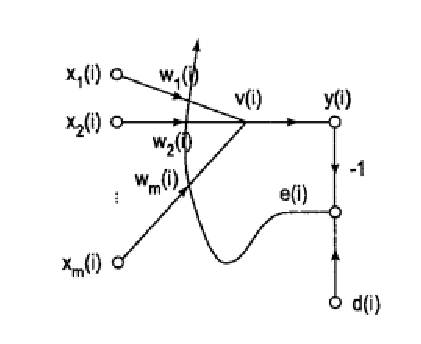
\includegraphics{signal.eps}
    \caption{Граф прохождения сигнала}
    \label{fig:signal}
\end{figure}

\begin{enumerate}
    \item Процесс фильтрации, предполагающий вычисление двух сигналов.
    \begin{itemize}
        \item Выходной сигнал, обозначаемый как y(i) и генерируемый в ответ на вектор входного воздействия \(x(i)\) с компонентами \(x_1(i),x_2(i),...,x_m(i)\).
        \item Сигнал ошибки, обозначаемый как \(e(i)\) и вычисляемый как отклонение выходного сигнала \(y(i)\) от выходного сигнала реальной системы \(d(i)\), который ещё называется целевым сигналом или ожидаемым откликом.
    \end{itemize}
    \item Процесс адаптации, включающий автоматическую подстройку синаптических весов нейрона на основе сигнала ошибки \(e(i)\).
\end{enumerate}
Комбинация этих двух процессов называется контуром с обратной связью нейрона. 
Учитывая линейность нейрона, выходной сигнал y(i) равен:
\[y(i) = \sum_{k=1}^m w_k(i)x_k(i),\]
где \(w_1(i),w_2(i,...,w_m(i)) - m \) синаптических весов нейрона, измеренных в момент времени \(i\). В матричной форме выходной сигнала \(y(i)\) можно представить, как скалярное произведение векторов \(w(i)\) и \(x(i)\):
\[y(i) = x^T(i)w(i),\] где \[w(i) = [w_1(i), w_2(i),...,w_m(i)]^T\]
Заметим, что индексация упрощённая и не содержит индекса, указывающего на конкретный нейрон, поскольку мы рассматриваем случай одного нейрона. Разность значения выходного сигнала нейрона и фактического выхода системы составляет сигнал ошибки:
\[e(i) = y(i) - d(i).\]

Для одного нейрона аналогом алгоритма обратного распространения является алгоритм минимизации среднеквадратической ошибки, основанный на использовании дискретных значений функции стоимости:
\[E(w) = 1/2e^2(n),\]
где \(e(n)\) - сигнал ошибки, измеренный в момент времени \(n\). Дифференцируя \(E(w)\) по вектору весов w, получим:
\[ \frac{\partial E(w)}{\partial w} = e(n) \frac{\partial e(n)}{\partial w } \]
Сигнал ошибки можно записать в следующем виде:
\[e(n) = d(n) - x^T(n)w(n).\]
Следовательно,
\[\frac{\partial e(n)}{\partial w(n)} = -x(n),\]
\[\frac{\partial E(w)}{\partial w(n)} = -x(n)e(n).\]
Используя полученный результат, можно оценить вектор градиента
\[ \hat g(n) = -x(n)e(n).\]
И используя последнюю формулу для вектора градиента в методе наискорейшего спуска, требуется сформулировать алгоритм минимизации среднеквадратической ошибки с следующем виде:
\[\hat w(n+1) = \hat w(n) +\eta x(n)e(n),\]
где \(\eta \) - параметр скорости обучения. 
При малых значениях \(\eta \) процесс обучения будет продвигаться медленно. При этом алгоритм минимизации среднеквадратичной ошибки будет запоминать большее количество предшествующих данных.
Тем самым на каждом шаге в ходе работы будет уменьшаться величина ошибки.
Данный классификатор может разделить обучающее множество на 2 класса: \(C_1\) и \(C_2\). Решающее правило сводится к следующему: входной сигнал относится к \(C_1\), если выходной сигнал равен 1, и к классу \(C_2\), если выход равен нулю. Входное множество разделится гиперплоскостью, определяемой формулой:
\[ \sum_{i=1}^m w_i x_i+b = 0 \]

\begin{figure}[t]
    \centering
    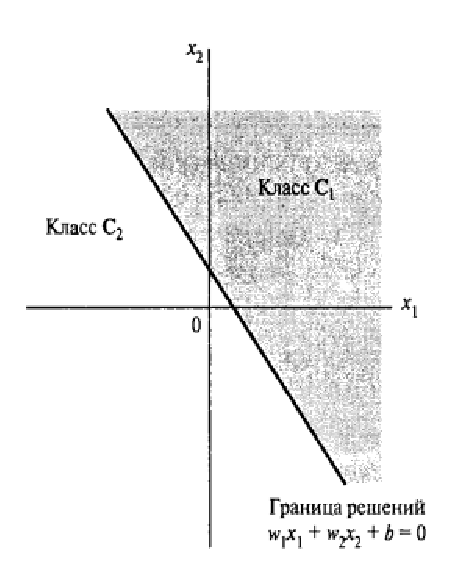
\includegraphics{c1c2.eps}
    \caption{Разделяющая плоскость для двумерного случая}
    \label{fig:c1c2}
\end{figure}

На рисунке \ref{fig:c1c2} это показано для случая двух переменных, \(x_1\) и \(x_2\), когда разделяющая гиперплоскость вырождается в прямую. Точки \((x_1,x_2)\), расположенные выше этой прямой, относятся к классу \(C_1\), а точки расположенные ниже, принадлежат классу \(C_2\). Синаптические веса корректируются согласно алгоритму минимизации среднеквадратической ошибки. Чтобы персептрон функционировал корректно, классы должны быть линейно-разделимыми.
В своей работе Розенблатт доказал, что данный алгоритм сходится и персептрон работает корректно для линейно-разделимых множеств с пороговой функцией активации. 
Далее были рассмотрены многослойные нейронные сети прямого распространения. Они имеют три отличительных признака.
\begin{enumerate}
    \item Каждый нейрон сети имеет нелинейную функцию активации. Данная функция является гладкой (дифференцируемой), в отличие от персептрона Розенблатта. самой популярной и используемой в данной работе является логистическая функция:
    \[y_i = \frac{1}{1+e^{-v_i}},\]
    где \(v_i\) сумма входных сигналов нейрона, а \(y_i\) - выход нейрона.
    \item Сеть содержит один или несколько слоёв скрытых нейронов, не являющихся частью входа или выхода сети. Эти нейроны позволяют сети обучаться решению сложных задач, последовательно извлекая наиболее важные признаки из входного вектора.
    \item Сеть обладает высокой степенью связности, реализуемой посредством синаптических соединений или их весовых коэффициентов.
\end{enumerate}
Еще стоит отметить, что производная логистической функции в определённой точке вычисляется от значения самой функции в той же точке:
\[ \phi'(x) = \phi(x)*(1-\phi(x)) \]

Пример полносвязной нейронной сети показан на рисунке \ref{fig:NN}. 
\begin{figure}[t]
    \centering
    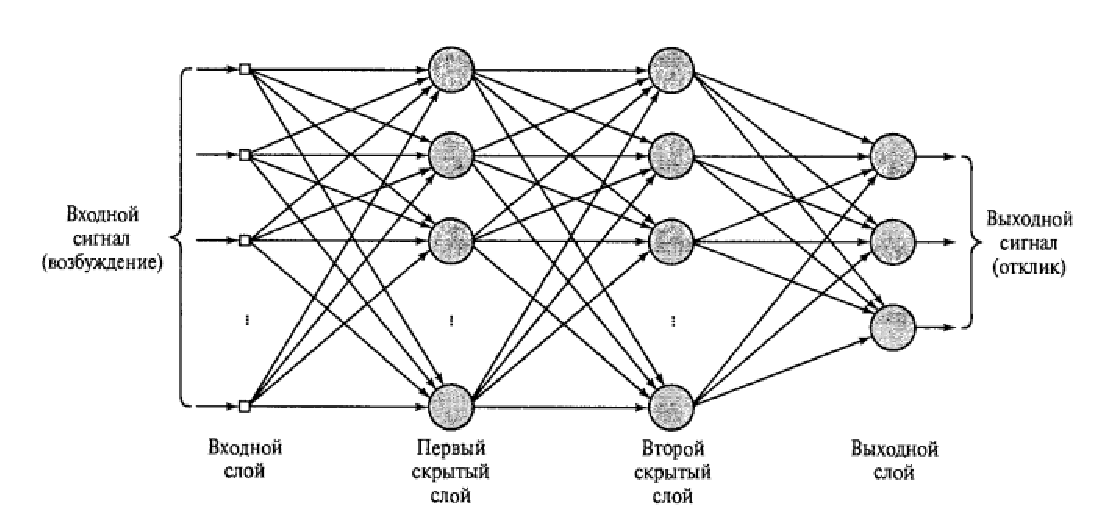
\includegraphics{NN.eps}
    \caption{Архитектурный граф многослойного персептрона с двумя скрытыми слоями}
    \label{fig:NN}
\end{figure}
Работа нейронной сети разделена на два типа вычислений.
\begin{enumerate}
    \item Прямой проход. Он считается от входного слоя по синапсам скрытых слоёв до выходного. При этом правила вычислений аналогичны вычислению однослойного персептрона.
    \item Обратный проход. Обратный проход идёт от выходного слоя к входному, распространяя ошибку и выполняя корректировку весов.
\end{enumerate}
Далее требуется рассмотреть более подробно алгоритм обратного распространения. Сначала произведём вычисление значения ошибки после прямого прохода. Оно вычисляется для каждого \(j\)-го нейрона выходного слоя в отдельности:
\[ e_j(n) = d_j(n) - y_j(n),\]
Общее значение энергии ошибки нейронной сети имеет вид:
\[ E(n) = \frac{1}{2}\sum_{j \in C}e^2_j(n),\]
где множество \(С\) содержит нейроны выходного слоя. Для каждого \(j\)-го нейрона следующее значение составляет его индуцированное локальное поле:
\[v_j = \sum^m_{i=0}w_{ji}(n)y_j(n),\]
где m - общее число входов (зи исключением порога) нейрона j. Синаптический вес \(w_{j0}\) равен порогу \(b_j\), применяемому к нейрону \(j\). Выход \(j\)-го нейрона равен
\[y_j(n) = \phi_j(v_j(n)).\]
Где \(\phi\) - активационная функция нейрона. Вообще говоря, они могут быть разные для разных нейронов в одной сети, но на практике мы будем использовать только логистическую функцию. Корректировать веса будем вычитанием из каждого веса по следующей величины:
\[\Delta w_{ij}(n) = - \psi \delta_j(n)y_j(n),\]
где локальный градиент \(\delta\) определяется выражением
\[\delta_j(n) = e_j(n)\phi_j'(v_j(n)) \]
Локальный градиент указывает на требуемое изменение синаптического веса. Как видно из формул ключевым фактором в вычислении величины коррекции является сигнал ошибки \(e_j(n)\) нейрона \(j\). В этом случае можно выделить два различных случая - выходной или скрытый нейрон. 
В первом случае величина ошибки известна, получается вычитанием желаемого отклика из фактического.
Во втором случае, происходит вычисление не значения ошибки, а сразу величины градиента скрытого нейрона по следующей формуле:
\[ \delta_j(n) = \phi_j'(v_j(n))\sum_k \delta_k(n)w_{kj}(n)\].

Критерием сходимости алгоритма обратного распространения ошибки является достаточно малая абсолютная интенсивность изменений среднеквадратической ошибки в течение эпохи, либо можно на каждом шаге проверять значение ошибки на тестовой выборке и остановится на достаточном уровне величины правильных ответов. При излишнем количестве выученных примеров есть возможность столкнуться с явлением переобучения.
\section{Алгоритмы оптимизации}
Далее приведены различные алгоритмы оптимизации для градиентного спуска.
Рассмотрим сложности, которые могут возникнуть при применении обучения  методом градиентного спуска:
\begin{itemize}
    \item Медленная скорость сходимости метода при малом шаге обучения и расходимость при большом шаге. Было бы удобно автоматически определять шаг обучения.
    \item Застревание в локальных минимумах функции ошибок. То есть, из-за медленной скорости шага по гиперплоскости ошибок почти невозможно проскочить локальные минимумы.
    \item Есть признаки, которые встречаются редко, но имеют особую значимость для классификации объекта. В методе градиентного спуска есть риск не заметить этот признак в общем потоке и дать ему, как и остальным малый вес.
    \item Существуют и обратная проблема, когда требуется найти важные признаки и не обращать внимания на случайные шумы.
\end{itemize}
Далее будут рассмотрены различные методы обучения нейронной сети. Для всех случаев будут разобраны плюсы и минусы метода, даны краткие формулы для применения. \\
\textbf{Метод стохастического градиента(SGD).}\\
Все его недостатки описаны выше, для сравнения с другими методами напишем только формулу обновления весов нейронной сети:
\[ w_{n+1} = w_n - \eta \delta_t,\]
где \(\delta_t\) - значение локального градиента.\\
\textbf{Метод стохастического градиента с инерцией(Nesterov Accelerated Gradient).}\cite{bib:nesterov} \\
Идея метода в том, что мы используем инерцию для того, чтобы ускорить движение по длинной пологой части гиперплоскости ошибок. Для этого требуется запоминать направление пройденное за последние несколько шагов, то есть воспользуемся экспоненциальным скользящим средним:
\[v_{t+1} = \eta v_t - \mu  \delta_t\]
\[w_{t+1} = w_t + v_{t+1}\]
Благодаря этому методу возможно ускорить нахождение оптимального решения. Также благодаря ускорению приобретённому во время движения по гиперплоскости ошибок, мы можем преодолеть локальные минимумы. А метод градиентный метод Нестерова отличается от предыдущего, что происходит заглядывание вперёд по вектору обновления, по следующей формуле:
\[v_{t+1} = \eta v_t - \mu  \nabla f(w_t + \eta v_t)\]
\[w_{t+1} = w_t + v_{t+1},\]
Где \(f(w_t + \eta v_t)\) - градиент функции потерь в уже обновлённой точке.
Такое изменение позволяет двигаться быстрее, если производная увеличивается. \\
\textbf{Метод адаптивного градиента (Adagrad).\cite{bib:Adagrad}}\\
Некоторые признаки могут быть крайне информативными, но встречаться редко. Особый графический узор, либо необычное слово. Требуется проверять насколько часто обновляется каждый параметр в отдельности, учитываю историю всех предыдущих градиентов. Идея масштабирования. Это делается с помощью деления каждого элемента в градиенте на квадратный корень суммы квадратов прошлых соответстующих элементов градиента. Формула пересчёта:
\[g_{t+1} = g_t + \nabla f(w_t)^2 \]
\[w_{t+1} = w_t - \frac{\mu \nabla f(w_t) }{\sqrt{g_{t+1} + \epsilon)} }  \] 
Здесь \(\epsilon\) требуется, чтобы не было ошибки деления на ноль. У часто обновляющегося в прошлом параметра значение \(g_t \) будет в знаменателе очень большим, там самым будет меняться меньше, чем у параметра, который поменялся меньше раз. Идея алгоритма в том, чтобы уменьшать обновление элементов, которые и так часто обновляются, и находить редкие параметры. Ещё одним достоинством Adagrad  является отсутствие необходмости точно подбирать скорость обучения. Его следует подбирать достаточно большим, потому что благодаря \(g_t\) автоматически происходит затухание скорости обучения, а после многих шагов алгоритм парализуется.

\textbf{Метод адаптивного скользящего среднего градиентов (RMSProp).\cite{bib:rmsprop}}\\
Метод похожа на Adagrad, только вместо полной суммы обновлений хранится экспоненциальное скользящее среднее::
\[g_{t+1} = \gamma g_t + (1-\gamma) \nabla f(w_t)^2 \]
\[w_{t+1} = w_t - \frac{\mu \nabla f(w_t) }{\sqrt{g_{t+1} + \epsilon)} }  \] 
Тем самым, больше шаг обучения со временем не уменьшается. Знаменатель это корень из среднего квадратов градиентов - Root Mean Square Propagation. Метод неопубликован, взят из курса лекций Geoff Hinton.\\
\textbf{Метод адаптивного шага обучения(Adadelta).\cite{bib:adadelta}}\\
Метод использует то же самое скользящее среднее что и RMSProp, но метод также также вычисляет скользящее среднее \(x_t\) по \(v_t\), аналогичными инерции, но при обновлении этой величина используется квадрат текущего шага:
\[g_{t+1} = \gamma g_t + (1-\gamma) \nabla f(w_t)^2 \]
\[v_{t+1} = - \frac{\sqrt{x_t + \epsilon \nabla f(w_t)}}{\sqrt{g_{t+1}+ \epsilon}}\]
\[x_{t+1} = \gamma x_t + (1 - \gamma) v^2_{t+1} \]
\[w_{t+1} = w_t + v_{t+1} \]
В данном случае получается эффект обратный Adagrad и RMSProp. Сильнее обновляются веса, которые используются чаще, потому что \(\nabla  w_t\) стал значимым, мы должны накопить большую сумму в числителе дроби. 
\\
\textbf{Метод адаптивной инерции (Adam).\cite{bib:adam}}
Метод адаптивной инерции сочетает в себе все идеи, описанные выше. Отличия следующие: оценка первого момента вычисляется как скользящее среднее, из-за того, что оценки первого и второго моментов инициализируются нулями, используется коррекция, чтобы результируюшие оценки не были смещены к нулю. Метод инвариантен к масштабированию градиентов. Правило пересчёта: 
\[m_{t+1} = \gamma_1 m_t + (1-\gamma_1) \nabla f(w_t) \]
\[g_{t+1} = \gamma_2 g_t + (1-\gamma_2) \nabla f(w_t)^2 \]
\[\hat{m}_{t+1} = \frac{m_{t+1}}{1 - \gamma^{t+1}_1} \]
\[\hat{g}_{t+1} = \frac{g_{t+1}}{1 - \gamma^{t+1}_2} \]
\[w_{t+1} = w_t - \frac{\mu \hat{m}_{t+1}}{\sqrt{\hat{g}_{t+1} + \epsilon}}\]



\chapter{Практическая часть}
\section{Вычислительный эксперимент} 
Для практического эксперимента в ходе работы рассмотрена задача определения рукописной цифры по изображению. Исходные данные взяты с открытой площадки для соревнований по машинному обучению \cite{kaggle:com}.
В процессе решения задачи был использован язык программирования Python 2.7.11, и его алгебраическая библиотека numpy \cite{numpy:package}.
В качестве исходных данных есть файл train.csv из обучающего примера "Digit Recognizer"\  размером 73.2 мбайта. В нём содержится 42000 размеченных примеров. Входной вектор состоит из 784 значений - черно-белое изображение 26*26 целых чисел от нуля до 255, чем больше значение, тем ярче пиксель. Первое число в каждой строке - метка числа от нуля до девяти.
Получается на вход сети будем подаваться вектор с 784 значениями, а на выходе имеется 10 нейронов, какой из них даёт наибольшее значение, тот и является выходным значением сети. Для удобства на выходе программы выводится только номер нейрона с наибольшим значением, то есть от нуля до девяти. 

Обучение происходит на 3/4 выборки (30000 примеров выбранных случайно), потом мы проверяем сеть на 1000 тестовых примеров взятых случайно. Также мы замеряем время обучения - в среднем оно происходит в пределах одной минуты. В это время не входит загрузка данных с диска, но также входит величина проверки на тестовой выборке, потому что она происходит почти мгновенно.

Каждый метод написан в отдельном модуле(файле), которые импортируется основной программой. Далее основная программа выполняет их по очереди с одинаковыми условиями.
Следует отметить, что результаты зависят от случайных значений, полученных при инициализации алгоритма, и во время перекрёстной проверки. 
Для сравнения алгоритмов оптимизации стохастического градиента во время вычислений встроена проверка\ttfamily accurance \normalfont. Чтобы увеличивать значительно время вычислений вычисление количества правильных ответов на тестовой выборке происходит каждый трёхсотый шаг. 
\section{Оценка результатов}
Приведены графики (\ref{fig:SGD} - \ref{fig:Adam}), где на оси Ох обозначен каждый трёхсотый шаг алгоритма, а на оси Оу процент правильных ответов.  

\begin{figure}[!hb]
    \centering
    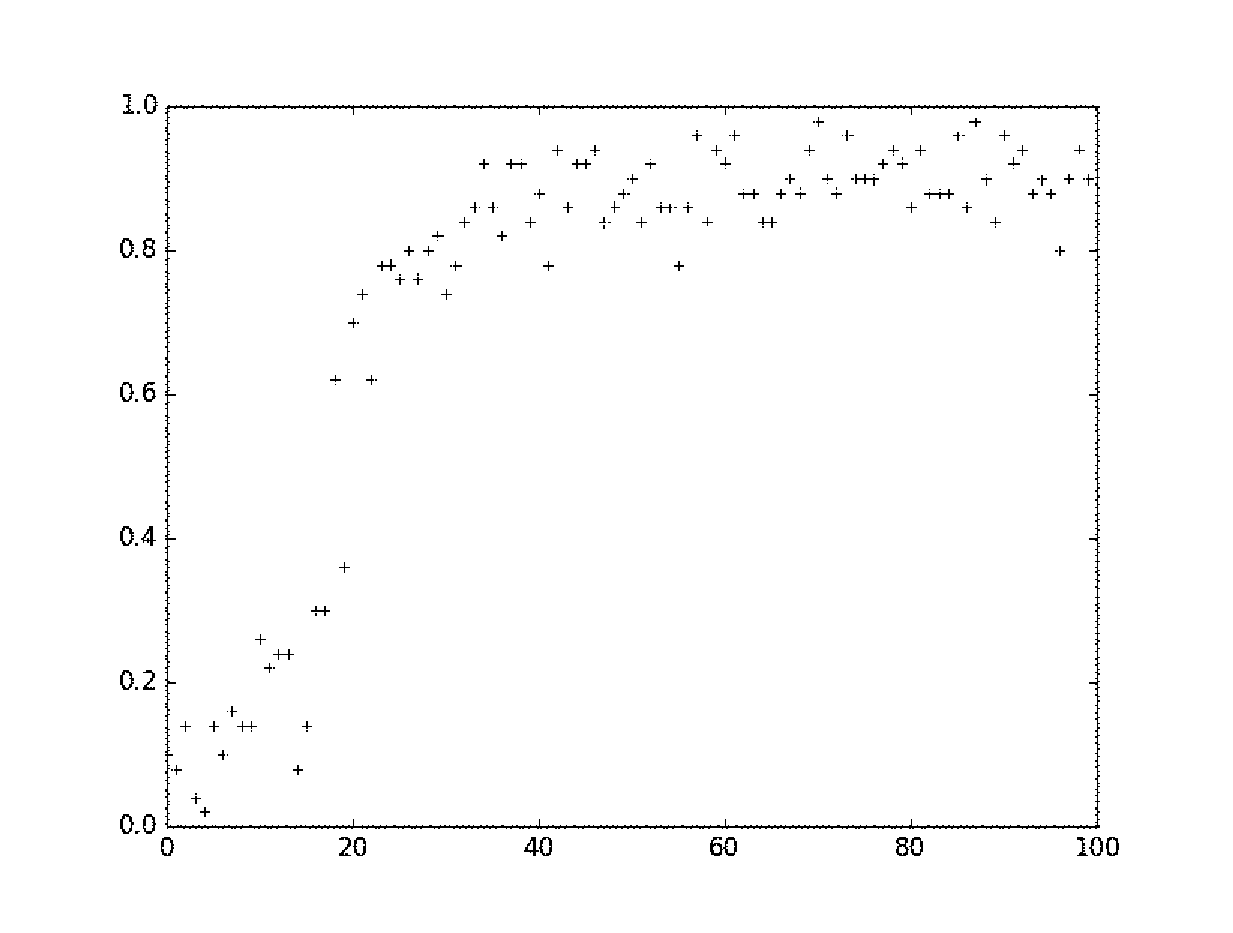
\includegraphics[width=1.0\textwidth]{SGD.eps}
    \caption{Метод стохастического градиента(SGD).}
    \label{fig:SGD}
\end{figure}
 
\begin{figure}
    \centering
    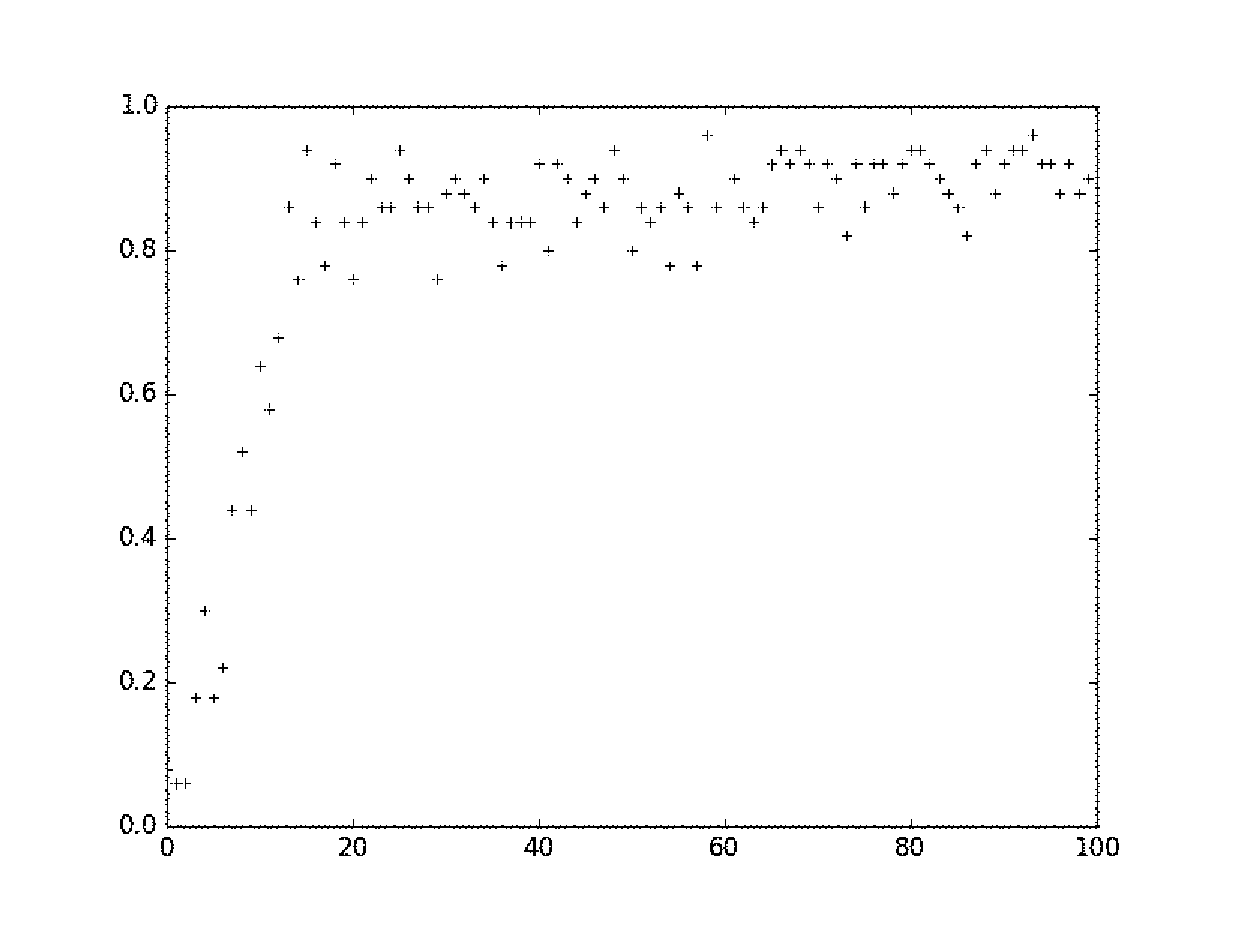
\includegraphics[width=1.0\textwidth]{Nesterov.eps}
    \caption{Метод стохастического градиента с инерцией(Nesterov Accelerated Gradient).}
    \label{fig:Nesterov}
\end{figure}

\begin{figure}
    \centering
    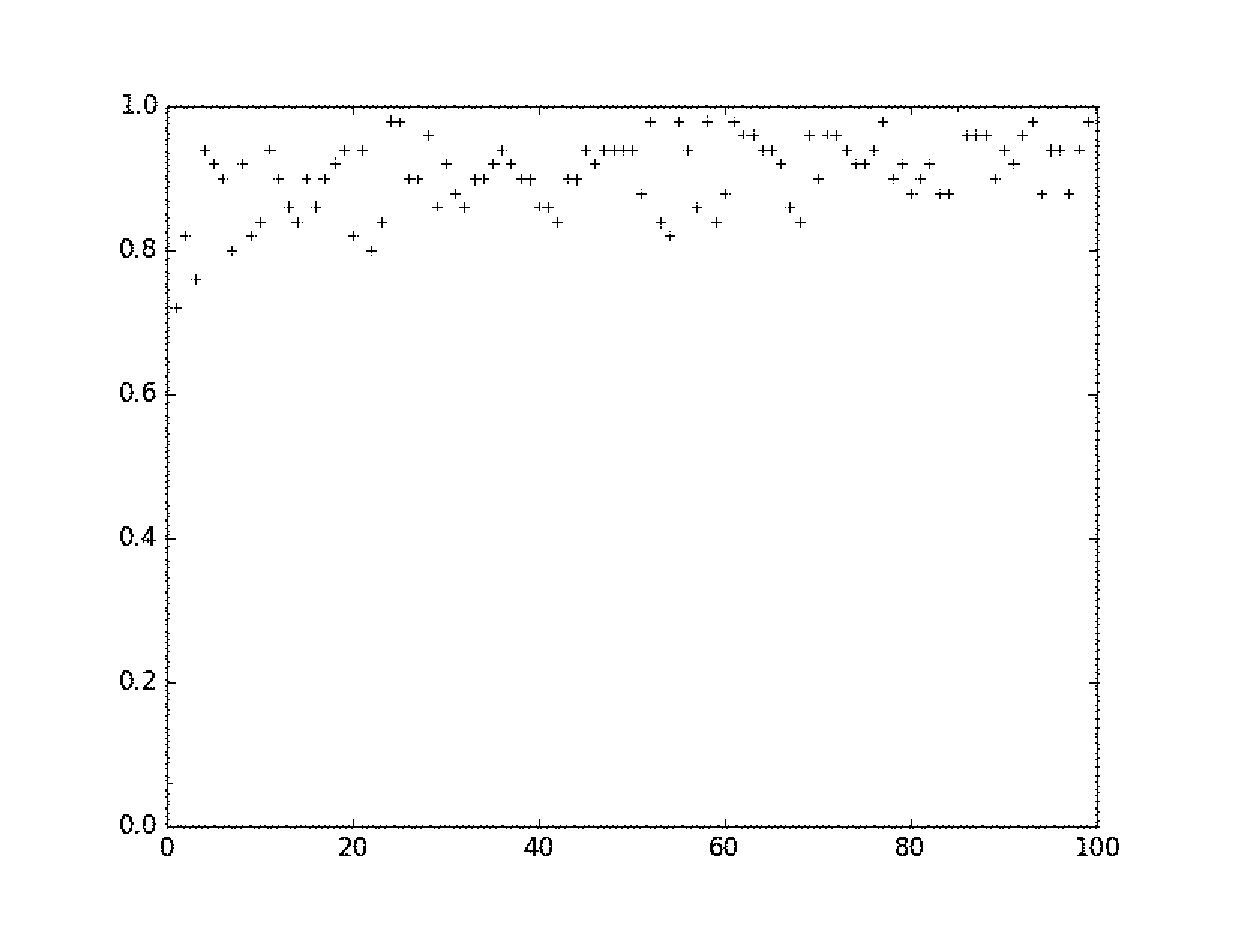
\includegraphics[width=1.0\textwidth]{Adagrad.eps}
    \caption{Метод адаптивного градиента (Adagrad).}
    \label{fig:Adagrad}
\end{figure}
 
\begin{figure}
    \centering
    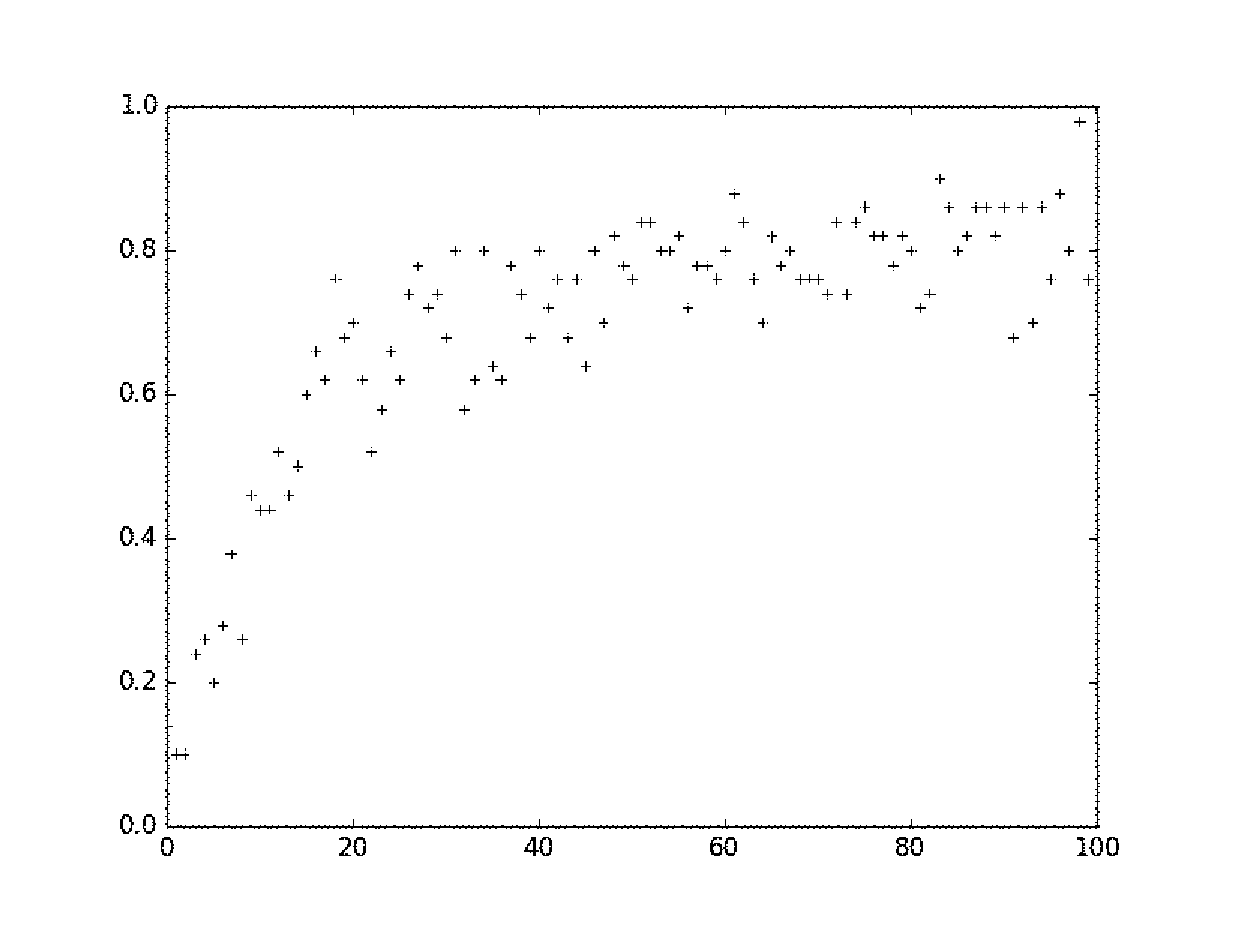
\includegraphics[width=1.0\textwidth]{RMSProp.eps}
    \caption{Метод адаптивного скользящего среднего градиентов (RMSProp).}
    \label{fig:RMSProp}
\end{figure}
 
\begin{figure}
    \centering
    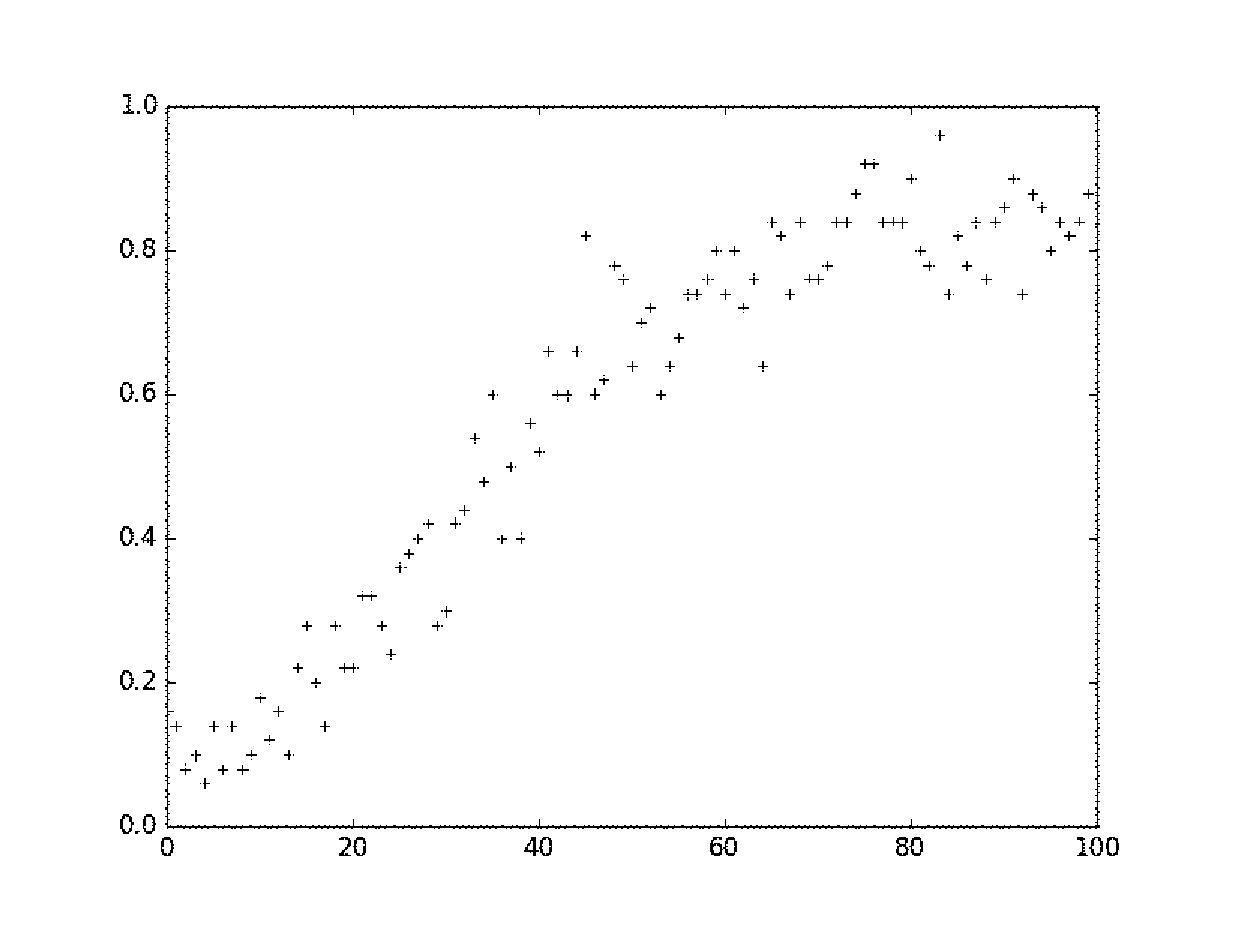
\includegraphics[width=1.0\textwidth]{Adadelta.eps}
    \caption{Метод адаптивного шага обучения(Adadelta).}
    \label{fig:Adadelta}
\end{figure}

\begin{figure}
    \centering
    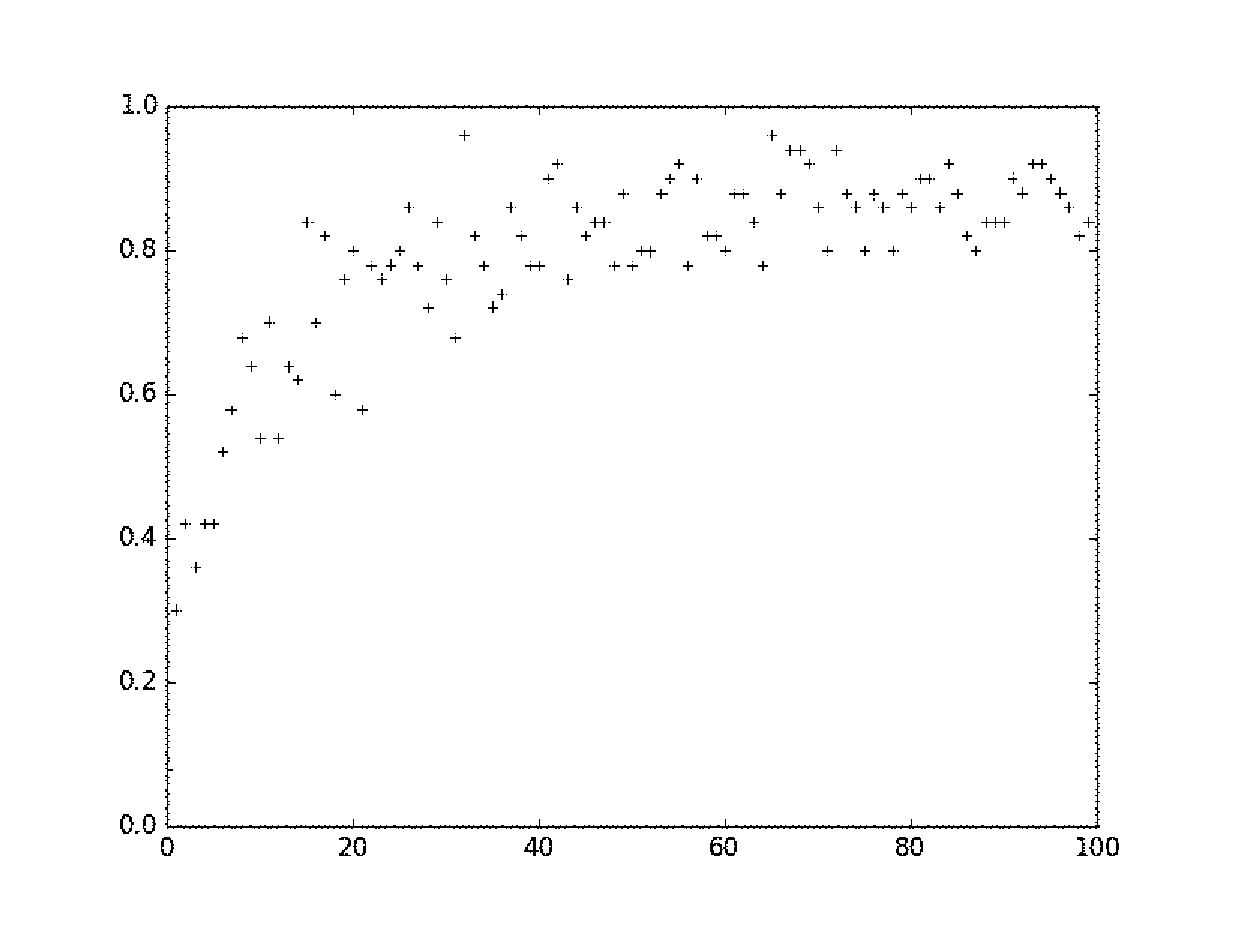
\includegraphics[width=1.0\textwidth]{Adam.eps}
    \caption{Метод адаптивной инерции (Adam).}
    \label{fig:Adam}
\end{figure}
\clearpage


Также приведём вывод программы для каждого метода оптимизации. В нём сначала написано название метода, потом время вычислений и процент правильных ответов на тестовой выборке, состоящей из тысячи примеров.

\begin{lstlisting}
    SGD
    time
    52.3459999561
    accurance: 0.899
    
    Nesterov
    time
    74.001999855
    accurance: 0.912
    
    Adagrad
    time
    89.3410000801
    accurance: 0.94
    
    RMSProp
    time
    92.371999979
    accurance: 0.843
    
    Adadelta
    time
    136.967000008
    accurance: 0.864
    
    Adam
    time
    176.016000032
    accurance: 0.872
\end{lstlisting}
\\
Как видно из рисунков, процент правильных ответов колеблется вокруг 90\%. Это происходит, потому что на каждой проверке тестовая выборка меняется, а на каких-то примерах результат может быть хуже чем на других. В основном уже после 3000 примеров\ttfamily accurance \normalfont становится более 95\%. При проведённых тестах наилучший результат показал метод \ttfamily Adagrad\normalfont. После проведения первых тестов значение \ttfamily accurance \normalfont достигло 0,7, а конечный результат составил 94\%, что на 3 процента больше, чем ближайший к нему метод. Также все алгоритмы с использованием момента инерции показали скорость обучения намного превосходящую изначальный алгоритм стохастического градиента.

Поскольку Adagrad показал себя лучше всех остальных алгоритмов, приведены несколько примеров изображений(\ref{fig:13931_6} - \ref{fig:909_7}), на которых ответ был неверным. При их просмотре не очевидно, какая цифра изображена на рисунке. Из этого можно заключить, что задача распознавания для подавляющего множества изображений решена верно. 

Увеличение скорости обучения и повышение его качества доказало целесообразность применения оптимизационных методов на практике.

\\ 
\begin{figure}[b]
    \centering
    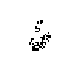
\includegraphics[width=1.0\textwidth]{13931_6.eps}
    \caption{Пример 13931, цифра 6.}
    \label{fig:13931_6}
\end{figure}
\\
%\ref{fig:1865_2}. 
\begin{figure}
    \centering
    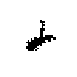
\includegraphics[width=1.0\textwidth]{1865_2.eps}
    \caption{Пример 1865, цифра 2.}
    \label{fig:1865_2}
\end{figure}
\\
%\ref{fig:6503_0}. 
\begin{figure}
    \centering
    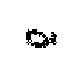
\includegraphics[width=1.0\textwidth]{6503_0.eps}
    \caption{Пример 6503 цифра 0.}
    \label{fig:6503_0}
\end{figure}
\\
%\ref{fig:909_7}. 
\begin{figure}
    \centering
    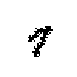
\includegraphics[width=1.0\textwidth]{909_7.eps}
    \caption{Пример 909 цифра 7.}
    \label{fig:909_7}
\end{figure}
\\
\\
\\


\chapter*{Заключение}
\addcontentsline{toc}{chapter}{\tocsecindent{Заключение}}
В рамках настоящей работы была рассмотрена задача выбора метода оптимизации алгоритма градиентного спуска для обучения нейронной сети на примере решения задачи распознавания арабских рукописных цифр. В начале работы приведены основные теоретические сведения об искусственных нейронных сетях, и об их обучении алгоритмом обратного распространения ошибки с помощью стохастического градиента. Далее в теоретической части рассмотрены следующие методы оптимизации алгоритма стохастического градиента:
\begin{itemize}
    \item Метод стохастического градиента с инерцией(Nesterov Accelerated Gradient).
    \item Метод адаптивного градиента (Adagrad).
    \item Метод адаптивного скользящего среднего градиентов (RMSProp).
    \item Метод адаптивного шага обучения(Adadelta).
    \item Метод адаптивной инерции (Adam).
\end{itemize}
Проведён анализ алгоритмов, включающий рассмотрение положительных и отрицательных сторон каждого метода. Разработана программа на языке Python 2.7.11. Задачу распознавания методом обратного распространения решить удалось с большим показателем точности равным в среднем 90\%. Далее проверен каждый метод оптимизации, среди них наилучший результат показал метод адаптивного градиента (Adagrad). Оценка методов происходила по следующим параметрам:
\begin{itemize}
    \item Cкорость обучения (по количеству пройденных эпох, требуемых для заданной точности).
    \item Отношение верных ответов в конце обучения на тестовой выборке.
\end{itemize}
Из теоретических предположений описанных в \cite{hykin:nn} можно сделать вывод, что для дальнейшего увеличения показателей сети может потребоваться увеличение количества скрытых слоёв, либо изменение архитектуры сети (свёрточные нейронные сети).

\begin{thebibliography}{00}
\addcontentsline{toc}{chapter}{\tocsecindent{Литература}}

\bibitem{bib:keras}
Keras - Deep Learning library
\href{https://keras.io/}{https://keras.io/}

\bibitem{bib:caffe}
Caffe - deep learning framework
\href{http://caffe.berkeleyvision.org/}{http://caffe.berkeleyvision.org/}

\bibitem {hykin:nn} С. Хайкин
\emph{Нейронные сети. Полный курс.}// Издательский дом "Вильямс"\ , 2006

\bibitem{bib:nesterov}
A. Botev, G. Lever, D. Barber Nesterov’s Accelerated Gradient and Momentum as approximations to Regularised Update Descent. // Department of Computer Science University College London. 2016
\bibitem{bib:Adagrad}
J. Duchi, E. Hazan, Y. Singer
Adaptive Subgradient Methods for Online Learning and Stochastic Optimization.//  Journal of Machine Learning Research 12 (2011) 2121-2159 Submitted 3/10; Revised 3/11; Published 7/11
\bibitem{bib:adadelta}
Matthew D. Zeiler Adadelta: an adaptive learning rate method.// Google Inc., USA 2New York University, USA. 2012
\bibitem{bib:adam}
D. P. Kingma, J. L. Ba Adam: a method for stochastic optimization.// Published as a conference paper at ICLR 2015
\bibitem{bib:overview}
An overview of gradient descent optimization algorithms
\href{http://sebastianruder.com/optimizing-gradient-descent/ 2016}{http://sebastianruder.com/optimizing-gradient-descent/ 2016}

\bibitem{bib:rmsprop}
G. Hinton Lecture 6e of his Coursera Class.
\href{"http://www.cs.toronto.edu/tijmen/csc321/slides/lecture_slides_lec6.pdf"}{http://www.cs.toronto.edu/~tijmen/csc321/slides/lecture\_slides\_lec6.pdf}

\bibitem {numpy:package} http://www.numpy.org/
\emph{NumPy is the fundamental package for scientific computing with Python.}

\bibitem {kaggle:com} https://www.kaggle.com
\emph{Digit Recognizer}

%\bibitem {archiv:opt} https://arxiv.org/abs/1511.01158v3
%\emph{Distributed Deep Learning for Question Answering} 

%\bibitem{1992}
%Matan O., Baird H., Bromley J., Burges C., Denker J., Jackel L., Le Cun Y., Pednault E., Satterfield W., Stenard C., Thompson T. Reading handwritten digits: a ZIP code recognition system // Computer.~--1992.~--V.25,N.7.~--P.59~--63.
%\bibitem{WC2007}
%Shah F., Yousaf K. Handwritten digit recognition using image processing and neural networks // Proceedings of the World Congress on Engineering.~--2007.~--V.1.
%\bibitem{chinese}
%Lu Y., Tan C., Shi P., Zhang K. Segmentation of handwritten chinese characters from destination addresses of mail pieces // International journal of pattern recognition and artificial intelligence.~--2002.~--V.16, N.1~--P.85~--96.
%\bibitem{IJCA2012}
%Aggarwal A., Rani R., Dhir R. Recognition of Devanagari handwritten numerals using gradient features and SVM // International journal of computer applications.~--2012.~--V.48, N.8.~--0975~--888.
%\bibitem{JCS2009} 
%Omari S., Sumari P., Al-Taweel S., Husain A. Digital recognition using neural network // Journal of computer science.~--2009.~--I.5, N.6~--P.427~--434.
%\bibitem{IJCA2011}
%Perwej Y., Chaturvedi A. Neural networks for handwritten english alphabet recognition // International journal of computer applications.~--2011.~--V.20, N.7.~--0975~--8887.

\end{thebibliography}


%%%%%%%%%%%%%%%%%%%%%%%%%%%%%%%%%%%%%%%%%%%%%%%%%%%%%%%%%%%%

%\appendix
\newcommand\Section[1]{
 \refstepcounter{section}
 \section*{\reggedright
 \arabic{chapter}.\Alph{section}. #1}
% \addcontentsline{toc}{section}{%
% \arabic{chapter}.\Alph{section}. #1}
 }
 
 \newcommand\Chapter[1]{
 \refstepcounter{chapter}
 \chapter*{
 \begin{huge}
  \textbf{\chaptername\  \arabic{chapter}\\}
 \end{huge}%
 \bigskip \bigskip
 \raggedright #1
 }
 \addcontentsline{toc}{chapter}{\arabic{chapter}. #1}
 } 

%\chapter*{Приложение}

%\refstepcounter{chapter}
%\addcontentsline{toc}{chapter}{\tocsecindent{Приложение}}
%\Section{Листинг сети с одним скрытым слоем}
%Последний вариант программы доступен по адресу \cite{git:W}.

%\lstinputlisting[language=Python]{testW.py}

%\Section{Листинг сети с двумя скрытыми слоями}
%Последний вариант программы доступен по адресу \cite{git:W2}.
%\lstinputlisting[language=Python]{testW2.py}


\end{document}
